\documentclass[12pt,a4paper]{article}
%setting margins
\usepackage[margin=1in]{geometry}

%%%%%%%%%%%%%%%%%%%%%%%%%%%%%%%%%%%%%%%%%%%%%%%%%%%%%%%%
%packages
\usepackage{amsmath}
\usepackage{blindtext}
\usepackage{fancyhdr}
\usepackage{enumerate}
\usepackage[shortlabels]{enumitem}
\usepackage{setspace}
\usepackage{tcolorbox}
\usepackage{pgfplots}
\usepackage{multicol}
\usepackage{subfiles} % Best loaded last in the preamble
\pgfplotsset{compat=1.18}
\usepackage{subcaption}
\usepackage{graphicx}
\usepackage[thinc]{esdiff}
%%%%%%%%%%%%%%%%%%%%%%%%%%%%%%%%%%%%%%%%%%%%%%%%%%%%%%%%
\pagestyle{fancy}
\fancyhead[l]{Rüzgar Erik}
\fancyhead[c]{Notes For the 12th Unit}
\fancyhead[r]{MATH104}
\fancyfoot[c]{\thepage}
\renewcommand{\headrulewidth}{0.2pt}
\setlength{\headheight}{15pt}
%%%%%%%%%%%%%%%%%%%%%%%%%%%%%%%%%%%%%%%%%%%%%%%%%%%%%%%%
%makes all equations centered use originalequation for normal mode
\let\originalequation\equation
\let\endoriginalequation\endequation

\renewenvironment{equation}
  {\begin{center}\originalequation}
  {\endoriginalequation\end{center}}


%%%%%%%%%%%%%%%%%%%%%%%%%%%%%%%%%%%%%%%%%%%%%%%%%%%%%%%%
%Define a new tcolorbox environment named "definition"
  \newtcolorbox{definitionbox}{
    colback=blue!5!white,
    colframe=blue!75!black,
    title=DEFINITION
  }
  
  \newenvironment{definition}{\begin{definitionbox}}{\end{definitionbox}\vspace{1\baselineskip}}

%%%%%%%%%%%%%%%%%%%%%%%%%%%%%%%%%%%%%%%%%%%%%%%%%%%%%%%%
\newcommand{\example}{\vspace{1\baselineskip}\par\noindent\textcolor{red}{EXAMPLE: }}
%%%%%%%%%%%%%%%%%%%%%%%%%%%%%%%%%%%%%%%%%%%%%%%%%%%%%%%%

%Define a new tcolorbox environment named "theorem"
\newtcolorbox{theorembox}{
    colback=red!5!white,
    colframe=red!75!black,
    title=THEOREM
  }
  
  \newenvironment{theorem}{\begin{theorembox}}{\end{theorembox}\vspace{1\baselineskip}}

%%%%%%%%%%%%%%%%%%%%%%%%%%%%%%%%%%%%%%%%%%%%%%%%%%%%%%%%

\newtcolorbox{corollarybox}{
    colback=blue!5!white,
    colframe=blue!75!black,
    title=Corollary
}
  
\newenvironment{corollary}{\begin{corollarybox}}{\end{corollarybox}\vspace{1\baselineskip}}


\newtcolorbox{rulebox}[1]{
    colback=red!5!white,
    colframe=red!75!black,
    title=#1
}

\newenvironment{ruleBox}[1]{\begin{rulebox}{#1}}{\end{rulebox}\vspace{1\baselineskip}}


%%%%%%%%%%%%%%%%%%%%%%%%%%%%%%%%%%%%%%%%%%%%%%%%%%%%%%%%

%Define a new tcolorbox environment named "theorem"

\newtcolorbox{note}{
    colback=white,
    colframe=black,
}

\newenvironment{mynote}{\vspace{1\baselineskip}\begin{note}}{\end{note}\vspace{1\baselineskip}}

%%%%%%%%%%%%%%%%%%%%%%%%%%%%%%%%%%%%%%%%%%%%%%%%%%%%%%%%



\newcommand{\lopital}{L'Hôpital's Rule }
\newcommand{\anc}{\(\{a_n\}\)}
\newcommand{\an}{\(a_n\)}
\newcommand{\infsum}{\sum_{n=1}^{\infty}}

\fancypagestyle{firstpage}{
    \fancyhf{} % Clear header and footer
    \renewcommand{\headrulewidth}{0pt} % Remove header rule
}

% Redefine \maketitle to include a fancy box
\makeatletter
\renewcommand{\maketitle}{%
  \thispagestyle{firstpage} % Apply the firstpage style for the first page
  \begin{tcolorbox}[colback=white,colframe=black,width=\textwidth,arc=0mm,auto outer arc]
    \begin{center}
      \Large \@title \\[1ex] \large \@date \\ \textit{Rüzgar ERİK}
    \end{center}
  \end{tcolorbox}
}
\makeatother


%%%%%%%%%%%%%%%%%%%%%%%%%%%%%%%%%%%%%%%%%%%%%%%%%%%%%%%%
\begin{document}



\title{Vector Valued Functions and Motions In Space}
\date{MATH 104}
\maketitle
\tableofcontents % This command generates the index page

\newpage % Start a new page for the content




\section{Vector Valued Functions and Motions In Space}

When a particle moves through space during a time interval \textit{I}, we think of the particle's coordinates as functions defined on \textit{I}.


\begin{center}
    \(x = f(t)\), \(y = f(t)\), \(z = f(t)\), \(t \in \mathit{I}.\)
\end{center}


\noindent The points \(\left(x, y, z\right) = \left(f(t), g(t), h(t)\right), t \in \mathit{I} \), make up the \textbf{curve} in space that we call the particle's \textbf{path}. The equations and interval parametrize the curve.

A curve in space can also be represented in vector form. The vector

    \[r(t) = \vec{OP} = f(t)\mathbf{i} + g(t)\mathbf{j} + h(t)\mathbf{k}\]
from the origin to the particle's position \(P(f(t),g(t),h(t))\) at time t is the particle's position vector. 
The functions are \textbf{component functions} of the position vector. We think of the particle's path as the curve traced bt \textbf{r} during the time interval \textit{I}.

A \textbf{vector-valued function} or \textbf{vector function} on a domain set \textit{D} is a rule that assigns a vector in space to each element in \textit{D}.

Real-valued functions are called scalar functions to distinguish them from vector
functions. The components of \textbf{r} are the scalar functions of \textit{t}. The domain of a vector-valued function is the common domain of its components.



\newpage

\begin{example}
Graph the vector function
\[r(t) = cos(t)\mathbf{i} + sin(t)\mathbf{j} + t\mathbf{k}\]
\end{example}

\noindent This vector function \textbf{r(\textnormal{t})} is defined for all real values of t. The curve traced by \textbf{r} winds around the circular cylinder\(x^2 + y^2 = 1\). The curve lied on the cylinder because \textbf{i \textnormal{and} j} components of \textbf{r}, being x- and y- coordinates of the tip of \textbf{r} satisfy the cylinder's equation:
\[ x^2 + y^2 = (\cos(t))^2 + (\sin(t))^2 = 1\]

The curve rises as the \textbf{k}-component \(z = t\) increases. Each time t increases by \(2\pi\), the curve completes one turn around the cylinder. The curve is called a \textbf{helix}.

The equations 
\[x = cos(t), y = sin(t), z = t\] 

parametrize the helix. 

\begin{figure}[h]
  \centering
  \begin{subfigure}[b]{0.3\textwidth} % Adjusted width and height
      \centering
      \resizebox{\linewidth}{!}{% helix_plot.tex


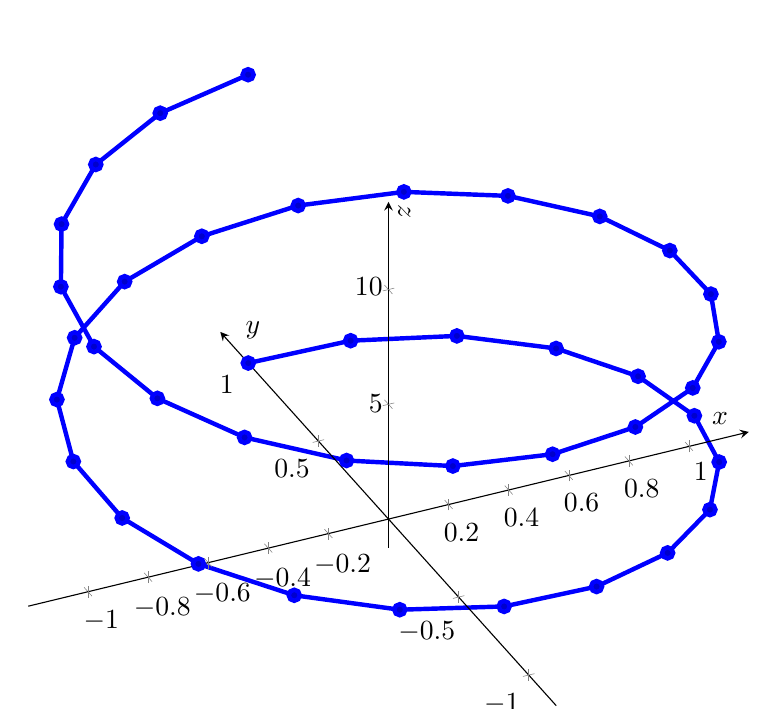
\begin{tikzpicture}
    \begin{axis}[
    axis lines=center,axis on top,
    colormap name=whitered,
    width=15cm,
    view={335}{50},
    enlargelimits=false,
    domain=-1:1,
    y domain=-1:1,
    samples=40, 
    xlabel=$x$,
    ylabel=$y$,
    zlabel={$z$},
    zlabel style={rotate=-90}, % Rotate z-label for better visibility
    every axis plot/.append style={ultra thick},
    enlarge x limits={0.1}, % Adjusted enlarge limits
    enlarge y limits={0.1}, % Adjusted enlarge limits
    enlarge z limits={0.1}% Adjusted enlarge limits % Increase plot thickness
    ]
        \addplot3+[domain=0:4*pi,samples y=0]
            ({sin(deg(x))},
             {cos(deg(x))},
             {x});
    \end{axis}
\end{tikzpicture}
} % Added \resizebox
      \caption{\(r(t) = \cos(t)\mathbf{i} + \sin(t)\mathbf{j} + t\mathbf{k}\)} % Corrected math notation
      \label{fig:plot1}
  \end{subfigure}
  \begin{subfigure}[b]{0.3\textwidth} % Adjusted width and height
      \centering
      \resizebox{\linewidth}{!}{
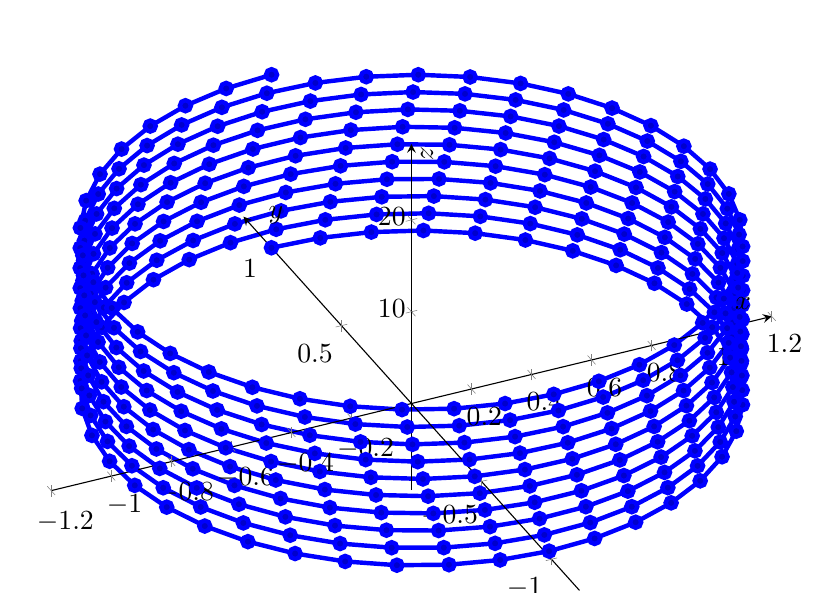
\begin{tikzpicture}
    \begin{axis}[
    axis lines=center,axis on top,
    colormap name=whitered,
    width=15cm,
    view={335}{50},
    enlargelimits=true,
    domain=0:20*pi, % Extend domain to cover multiple cycles
    y domain=-1:1,
    samples=400, 
    xlabel=$x$,
    ylabel=$y$,
    zlabel={$z$},
    zlabel style={rotate=-90}, % Rotate z-label for better visibility
    every axis plot/.append style={ultra thick},
    enlarge x limits={0.1}, % Adjusted enlarge limits
    enlarge y limits={0.1}, % Adjusted enlarge limits
    enlarge z limits={0.5}% Adjusted enlarge limits % Increase plot thickness
    ]
        \addplot3+[samples y=0]
            ({sin(deg(x))},
             {cos(deg(x))},
             {0.3*x});
    \end{axis}
\end{tikzpicture}

} % Added \resizebox
      \caption{\(r(t) = \cos(t)\mathbf{i} + \sin(t)\mathbf{j} + 0.3t\mathbf{k}\)} % Corrected math notation
      \label{fig:plot2}
  \end{subfigure}
  \begin{subfigure}[b]{0.3\textwidth} % Adjusted width and height
    \centering
    \resizebox{\linewidth}{!}{% helix_plot.tex


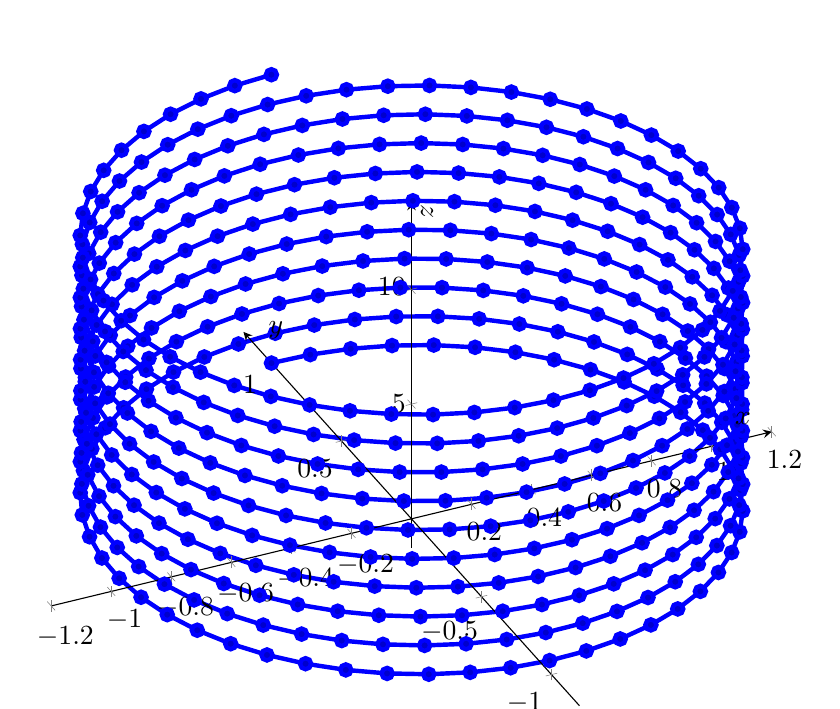
\begin{tikzpicture}
    \begin{axis}[
    axis lines=center,axis on top,
    colormap name=whitered,
    width=15cm,
    view={335}{50},
    enlargelimits=false,
    domain=-1:1,
    y domain=-1:1,
    samples=500, 
    xlabel=$x$,
    ylabel=$y$,
    zlabel={$z$},
    zlabel style={rotate=-90}, % Rotate z-label for better visibility
    every axis plot/.append style={ultra thick},
    enlarge x limits={0.1}, % Adjusted enlarge limits
    enlarge y limits={0.1}, % Adjusted enlarge limits
    enlarge z limits={0.1}% Adjusted enlarge limits % Increase plot thickness
    ]
        \addplot3+[domain=0:4*pi,samples y=0]
            ({sin(deg(5*x))},
             {cos(deg(5*x))},
             {x});
    \end{axis}
\end{tikzpicture}
} % Added \resizebox
    \caption{\(r(t) = \cos(5t)\mathbf{i} + \sin(5t)\mathbf{j} + t\mathbf{k}\)}
    \label{fig:plot3} % Changed label to avoid duplication
  \end{subfigure}
  \caption{Multiple helix plots side by side}
  \label{fig:multiplot}
\end{figure}

\newpage

\subsection{Limits and Continuity}

\begin{definition}
  Let \(\mathbf{r(t)} = f(t)\mathbf{i} + g(t)\mathbf{j} + h(t)\mathbf{k}\) be a vector function with domaiN \textit{D}, and \textbf{L} be a vector. We say that \textbf{r} has \textbf{limit L} as \textit{t} approaches \(t_0\) and write

  \[\lim_{t \to t_0} \mathbf{r}(t) = \mathbf{L}\]

\end{definition}

If \(\mathbf{L} = \mathit{L}_1\mathbf{i} + \mathit{L}_2\mathbf{j} + \mathit{L}_3\mathbf{k}\) then it can be shown that \(\lim_{t \to t_0} \mathbf{r}(t) = \mathbf{L}\) precisely When

\[\lim_{t \to t_0} f(t) =L_1, \lim_{t \to t_0} G(t) = L_2 , \lim_{t \to t_0} h(t) = L_3\]

\begin{example}
  If \(\mathbf{r}(t) = \cos(t)\mathbf{i} + \sin(t)\mathbf{j}+ t\mathbf{k}\) then

  \begin{align}
    \lim_{t \to \frac{\pi}{4}}\mathbf{r}(t) &= \left(\lim_{t \to \frac{\pi}{4}}\cos(t)\right)\mathbf{i} + \left(\lim_{t \to \frac{\pi}{4}}\sin(t)\right)\mathbf{j}+ \left(\lim_{t \to \frac{\pi}{4}}t\right)\mathbf{k} \\
    &=\frac{\sqrt{2}}{2}\mathbf{i} + \frac{\sqrt{2}}{2}\mathbf{j} + \frac{\pi}{4}\mathbf{k}
\end{align}

\begin{definition}
  A vector function \(\mathbf{r}(t)\) is \textbf{continious at a point} \(t = t_0\) in its domain if \(\lim_{t \to t_0} \mathbf{r}(t) = \mathbf{r}(t_0)\).
  The function is \textbf{continious} if it is continious at every point in its domain.
\end{definition}

\subsection{Derivatives and Motion}

Suppose that \(\mathbf{r(t)} = f(t)\mathbf{i} + g(t)\mathbf{j} + h(t)\mathbf{k}\) is the position vector of  a particle moving along a curve in space and that f, g, h, are differentiable functions of t.
Then the difference between the particle's position at time \(t\) and time \(t + \Delta t\) is the vector

\[\Delta \mathbf{r} = \mathbf{r}(t + \Delta t) - \mathbf{r}(t)\]



{\small
\[
\lim_{\Delta t \to 0}\frac{\Delta \mathbf{r}}{\Delta t} = \left[\lim_{\Delta t \to 0}\frac{f(t + \Delta t) - f(t)}{\Delta t}\right] \mathbf{i} + \left[\lim_{\Delta t \to 0}\frac{g(t + \Delta t) - g(t)}{\Delta t}\right] \mathbf{j} + \left[\lim_{\Delta t \to 0}\frac{h(t + \Delta t) - h(t)}{\Delta t}\right] \mathbf{k}
\]
}

\[= \left[\frac{\mathrm{d}f}{\mathrm{d}t}\right]\mathbf{i} + \left[\frac{\mathrm{d}g}{\mathrm{d}t}\right]\mathbf{j}+ \left[\frac{\mathrm{d}h}{\mathrm{d}t}\right]\mathbf{k}\]


\end{example}

\newpage

\begin{definition}
  The vector function \(\mathbf{r(t)} = f(t)\mathbf{i} + g(t)\mathbf{j} + h(t)\mathbf{k}\) has a \textbf{derivative at t} if f, g and h have Derivatives at t. The derivative is the vector function
  
  \[\mathbf{r}' = \frac{\mathrm{d}\mathbf{r}}{\mathrm{d}t} = \lim_{\Delta t \to 0} \frac{\mathbf{r}(t + \Delta t) - \mathbf{r}(t)}{\Delta t} = \frac{\mathrm{d}f}{\mathrm{d}t}\mathbf{i} + \frac{\mathrm{d}g}{\mathrm{d}t}\mathbf{j} + \frac{\mathrm{d}h}{\mathrm{d}t}\mathbf{k}\]  
\end{definition}

\noindent  A vector function \textbf{r} is \textbf{differentiable} if it is differentiable at every point of its domain. 

\noindent The curve traced by \textbf{r} is \textbf{smooth} if d\textbf{r}/dt is \textbf{continious} and \textbf{NEVER 0}.
\noindent A curve that is made up of finite number of smooth curves pieced together in a continious fashion is called \textbf{piecewise smooth}.



\begin{definition}
  If \textbf{r} is the position vector of a particle moving along a smooth curve in space then,

  \[\mathbf{v}(t) = \frac{\mathrm{d}\mathbf{r}}{\mathrm{d}t}\]
  is the particle's \textbf{velocity vector}, tangent to the curve. At any time t, the direction of \textbf{v} is the \textbf{direction of motion}, the magnitude of \textbf{v} is the particle's \textbf{speed}, and the derivative \textbf{a} = d\textbf{v}/dt, when it exists, it is the particle's \textbf{acceleration vector}.
\end{definition}


\begin{ruleBox}{Differentiation Rules for Vector Functions}
\begin{enumerate}
  \item Dot Product Rule: \(\frac{\mathrm{d}}{dt}\left[\mathbf{u}(t)\cdot\mathbf{v}(t)\right] = \mathbf{u}'(t)\cdot \mathbf{v}(t) + \mathbf{v}'(t)\cdot\mathbf{u}(t)\)
  \item Cross Product Rule: \(\frac{\mathrm{d}}{dt}\left[\mathbf{u}(t)\times\mathbf{v}(t)\right] = \mathbf{u}'(t)\times \mathbf{v}(t) + \mathbf{v}'(t)\times\mathbf{u}(t)\)
\end{enumerate}
\end{ruleBox}


\subsection{Vector Functions of Constant Lenght}

\begin{mynote}
If \textbf{r} is a differentiable vector function of \textit{t} and the lenght of \(\mathbf{r}(t)\) is consistant, then
\[\mathbf{r}\cdot \frac{\mathrm{d}\mathbf{r}}{\mathrm{d}t} = 0\]
\end{mynote}
\newpage
\section{Integrals of Vector Functions; Projectile Motion}

\subsection{Integrals of Vector Functions}

A differentiable vector function \textbf{R}(\textit{t}) is an \textbf{antiderivative} of a vector function \(\mathbf{r}(t)\) on an interval \textit{I} if d\textbf{R}/dt = \textbf{r} at each point of \textit{I}. 
The set of all antiderivatives on \textbf{r} on \textit{I} is the \textbf{indefinite integral} of \textbf{r} on \textit{I.}

\begin{definition}
  
  The \textbf{indefinite integral} of \textbf{r} with respect to \textit{t} is the set of all antiderivatives of \textbf{r} denoted by \(\int \mathbf{r}(t)\)
  \[\int\mathbf{r}(t)\mathrm{d}t = \mathbf{R}(t) + \mathbf{C}.\].



\end{definition}

\begin{definition}
  If the components of \(\mathbf{r(t)} = f(t)\mathbf{i} + g(t)\mathbf{j} + h(t)\mathbf{k}\) are integrable over \([a,b]\),
  then so is \textbf{r} and the \textbf{definite integral} of \textbf{r} from a to b is

  \[
    \int_{a}^{b}\mathbf{r}(t)\mathrm{d}t = \left(\int_{a}^{b} f(t)\mathrm{d}t \right)\mathbf{i} + \left(\int_{a}^{b} g(t)\mathrm{d}t \right)\mathbf{j} + \left(\int_{a}^{b} h(t)\mathrm{d}t \right)\mathbf{k}
    \]
    


\end{definition}

\subsection{The Vector and Parametric Equations for Ideal Projectile Motion}

If \(v_0\) makes an angle \(\alpha\) with the horizontal, then
\[\mathbf{v}_0 = (|\mathbf{v}_0|\cos\alpha)\mathbf{i} +(|\mathbf{v}_0|\sin\alpha)\mathbf{j} \]

Newton's second law of motion says that the force acting on the projectile is equal to the projectile's m times its acceleration (m\(\frac{\mathrm{d}^2r}{\mathrm{d}t^2}\)).
If force is solely the gravitational force \(-mg\mathbf{j}\) then,

\[m \frac{\mathrm{d}^2\mathbf{r}}{\mathrm{d}t^2} = -mg\mathbf{j} \quad \mathrm{and} \quad \frac{\mathrm{d}^2\mathbf{r}}{\mathrm{d}t^2} = -g\mathbf{j}\]


where g is the acceleration due to gravity. We find \textbf{r} as a function of \textit{t} by solving the initial value problem.

\begin{center}
  Differential equation: \(\frac{\mathrm{d}^2\mathbf{r}}{\mathrm{d}t^2} = -g\mathbf{j}\)
\end{center}

\begin{center}
  Initial Conditions: \(r = r_0\) and \(\frac{\mathrm{d}\mathbf{r}}{\mathrm{d}t}=v_0 \) when \(\mathit{t} = 0\)
\end{center}

The first integration gives

\[\frac{\mathrm{d}\mathbf{r}}{\mathrm{d}t} = -(gt)\mathbf{j} + v_0\]

And the second integration gives

\[r = -\frac{1}{2}gt^2\mathbf{j} + v_{0}t + r_0 \]

Substituting values of $v_0$ and $r_0$ from given initial conditions gives

\[r = -\frac{1}{2}gt^2\mathbf{j} + (v_0\cos\alpha)t\mathbf{i} + (v_0\sin\alpha)t\mathbf{j} + 0 \]


\begin{mynote}
  \textcolor{blue}{Ideal Projectile Motion Equation}

  \[r = (v_0\cos\alpha)t\mathbf{i} + \left((v_0\sin\alpha)t - \frac{1}{2}gt^2\right)\mathbf{j} \]


\end{mynote}

\begin{mynote}
  \textcolor{blue}{\textbf{Height, Flight Time and Range for Ideal Projectile Motion}}
  
  \begin{align*}
    \text{Maximum Height:} \quad y_{\text{max}} &= \frac{{(v_0 \sin\alpha)}^2}{2g}\\
    \text{Flight Time:} \quad t &= \frac{2v_0 \sin\alpha}{g}\\
    \text{Range:} \quad R &= \frac{{v_0}^2}{g}\sin(2\alpha)\\
  \end{align*}
\end{mynote}

\newpage

\section{Arc Lenght in Space}

\subsection{Arc Lenght Along a Space Curve}

\begin{definition}
  The \textbf{lenght} of a smooth curve \(\mathbf{r}(t) = x(t)\mathbf{i}+ y(t)\mathbf{j} + \mathbf{z}(t)\) \(a \geq t \geq b\), that is traced exactly once as t increases from \(t=a\) to \(t=b\) is
  \[\mathit{L} = \int_{a}^{b}\sqrt{\left(\frac{\mathrm{d}x}{\mathrm{d}t}\right)^2+\left(\frac{\mathrm{d}y}{\mathrm{d}t}\right)^2+\left(\frac{\mathrm{d}z}{\mathrm{d}t}\right)^2}\]
\end{definition}

The squere root in the definition of lenght is \(|\mathbf{v}|\), the lenght of velocity vector \(\mathrm{d}\mathbf{r}\slash \mathrm{d}t\). This enables us to write the formula for lenght in a shorter way.

\begin{ruleBox}{Arc Lenght Formula}

  \[\mathit{L} = \int_{a}^{b}|\mathbf{v}| \mathrm{d}t\]

\end{ruleBox}


If we choose a base point \(P(t_0)\) on a smooth curve \textit{C} parametrized by \textit{t}, each value of t determines a point \(P(t) = (x(t),y(t),z(t))\) on c and a "directed distance"

\[s(t) = \int_{t_0}^{t}|\mathbf{v}(\tau)\mathrm{d}\tau|\]

measured along \textit{C} from the base point. This is the arc  lenght formula for plane curves that have no z-component. If \(t>t_0\), \(s(t)\) is the distance along the curve from \(P(t_0)\) to \(P(t)\). If \(t < t_0\) is the negative of the distance.
Each value of \textit{s} determines a point on \textit{C}, and this parametrizes \textit{C} with respect to \textit{s}. We call \textit{s} an \textbf{arc lenght parametrer} for the curve. 

\begin{ruleBox}{Arc Lenght with Base Point \(P(t_0)\)}

  \[s(t) = \int_{t_0}^{t}\sqrt{\left[x'(\tau)\right]^2+\left[y'(\tau)\right]^2+\left[z'(\tau)\right]^2} = \int_{t_0}^{t}|\mathbf{v}(\tau)|\mathrm{d}\tau\]
\end{ruleBox}

If a curve \(\mathrm{r}(t)\) is already given in terms of some parameter \(t\) and \(s(t)\) is the arc lenght function given, then we may be able to solve for t as a function of \(s: t = t(s)\). Then the curve can be reparametrized in terms of s by substituting for \(t: \mathbf{r} = \mathbf{r}(t(s))\). The new parametrization identifies a point on the curve with its directed distance along the curve from the base point.

\newpage

\begin{example}
  This is an example for which we can actually find the arc lenght parametrization of a curve. If \(t_0=0\), the arc lenght parameter along the helix
  \[\mathbf{r}(t)=(\cos(t))\mathbf{i}+(\sin(t))\mathbf{j}+t\mathbf{k}\]
  from \(t_0\) to t is
  \begin{align*}
    s(t) &= \int_{t_0}^{t}|\mathbf{v}(\tau)|\mathrm{d}\tau\\
    &= \int_{t_0}^{t}\sqrt{2}\mathrm{d}\tau\\
    &= \sqrt{2}t
  \end{align*}

  Solving this equation for t gives \(t = \frac{s}{\sqrt{2}}\). Substituting into the position vector \textbf{r} gives the following arc lenght parametrization for the helix
  \[\mathbf{r}(t(s)) = \left(\cos\left(\frac{s}{\sqrt2}\right)\right)\mathbf{i} + \left(\sin\left(\frac{s}{\sqrt2}\right)\right)\mathbf{j}  + \frac{s}{\sqrt2}\mathbf{k}\]
  
\end{example}

\subsection{Speed on a Smooth Curve}

\begin{mynote}
  \[\frac{\mathrm{d}s}{\mathrm{d}t} = |\mathbf{v}(t)|\]
\end{mynote}

The equation says that the speed with which a particle moves along its path is the magnitude of \textbf{v}. Although the base point $P(t_0)$ plays a role in defining \(s\) in the arc lenght formula with base point it plays no role here. 
The rate at whichn a moving particle covers distance along its path is independent of how far it is away from the base point.

Notice that \(\frac{\mathrm{d}s}{\mathrm{d}t} > 0\) since, by definition \(|\mathbf{v}|\) is never zero for a smooth curve.

\subsection{Unit Tangent Vector}

We already know that the velocity vector \(v = \frac{\mathrm{d}\mathbf{r}}{\mathrm{d}t}\) is tangent to the curve \(\mathbf{r}(t)\) and the vector
\[\mathbf{T} = \frac{\mathbf{v}}{|\mathbf{v}|}\]
is therefore a unit vector tangent to the smooth curve, called the \textbf{unit tangent vector}. The unit tangent vector \textbf{T} is a differentiable function of \textit{t} whenever \textbf{v} is a differentiable function of\textit{t}. 

\newpage

\section{Curvature and Normal Vectors of a Curve}
\subsection{Curvature of a Plane Curve}

As a particle moves along a smooth curve in the plane, $\mathbf{T} = \frac{\mathrm{d}\mathbf{r}}{\mathrm{d}s}$ turns as the curve bends. Since $\mathbf{T}$ is a unit vector, its length remains constant and only its direction changes as the particle moves along the curve. The rate at which $\mathbf{T}$ turns per unit of length along the curve is called the \textit{curvature}. The traditional symbol for the curvature function is the Greek $\kappa$ ("kappa").

\begin{definition}
  If $\mathbf{T}$ is the unit vector of a smooth curve, the \textbf{curvature} function of the curve is
  \[\mathbf{\kappa} = \left|\frac{\mathrm{d}\mathbf{T}}{\mathrm{d}s}\right|\]

\end{definition}

If $\left|\frac{\mathrm{d}\mathbf{T}}{\mathrm{d}s}\right|$ is large, $\mathbf{T}$ turns sharply as the particle passes through $P$, and the curvature at $P$ is large. If $\left|\frac{\mathrm{d}\mathbf{T}}{\mathrm{d}s}\right|$ is close to zero, $\mathbf{T}$ turns more slowly and the curvature at $P$ is smaller.

If a smooth curve $\mathbf{r}(t)$ is already given in terms of some parameter other than the arc length parameter $s$, we can calculate the curvature as

\[\kappa = \left|\frac{\mathrm{d}\mathbf{T}}{\mathrm{d}s}\right| = \left|\frac{\mathrm{d}\mathbf{T}}{\mathrm{d}t}\frac{\mathrm{d}t}{\mathrm{d}s}\right|\]
\[= \frac{1}{\left|\frac{\mathrm{d}s}{\mathrm{d}t}\right|}\left|\frac{\mathrm{d}\mathbf{T}}{\mathrm{d}t}\right|\]
\[= \frac{1}{|v|}\left|\frac{\mathrm{d}\mathbf{T}}{\mathrm{d}t}\right|\]


\begin{ruleBox}{Formula for Calculating Curvature}

  If \(\mathbf{r}(t)\) is a smooth curve, then the curvature is the scalar function

  \[\kappa = \frac{1}{|\mathbf{v}|}\left|\frac{\mathrm{d}\mathbf{T}}{\mathrm{d}t}\right|\]
  Where \(\mathbf{T} = \frac{\mathbf{v}}{|\mathbf{v}|}\)  
\end{ruleBox}
\newpage

\begin{example}
  Here we find the curvature of a circle. We begin with the parametrization
  \[\mathbf{r}(t) = (a \cos t)\mathbf{i} + (a \sin t)\mathbf{j}\]
  of a circle of radius \(a\). Then,
  \[\mathbf{v} = \frac{\mathrm{d}\mathbf{r}}{\mathrm{d}t} = -(a \sin t)\mathbf{i} + (a \cos t)\mathbf{j}\]
  \[|\mathbf{v}| = \sqrt{(-a \sin t)^2 + (a \cos t)^2} = \sqrt{a^2} = a\]
  From this we find
\begin{align*}
  \mathbf{T} &= \frac{\mathbf{v}}{|v|} = -(\sin t)\mathbf{i} + (\cos t)\mathbf{j}\\
  \frac{\mathrm{d}\mathbf{T}}{\mathrm{d}t} &= -(\cos t)\mathbf{i} - (\sin t)\mathbf{j} \\
  \left|\frac{\mathrm{d}\mathbf{T}}{\mathrm{d}t}\right| &= 1
\end{align*}
Hence, for any value of the parameter \textit{t} the curvature of the circle is
\[\kappa = \frac{1}{|\mathbf{v}|}\left|\frac{\mathrm{d}\mathbf{T}}{\mathrm{d}t}\right| = \frac{1}{a}\]

\end{example}

Among the vectors orthogonal to the unit tangent vector \textbf{T}, there is one of particular significance because it points int the direction which the space curve is turning.
Since \textbf{T} has constant lenght, the derivative \(\mathrm{d}\mathbf{T}\slash\mathrm{d}s\) is orthogonal to \textbf{T}. Therefore id we divide \(\mathrm{d}\mathbf{T}\slash\mathrm{d}s\) by its lenght \(\kappa\) we obtain a unit vector \textbf{N} orthogonal to \textbf{T}

\begin{definition}
  At point where \(\kappa \neq 0\), the \textbf{principal unit normal} vector for a smooth curve in the plane is
  \[\mathbf{N} = \frac{1}{\kappa} \frac{\mathrm{d}\mathbf{T}}{\mathrm{d}s}\]
\end{definition}

The vector \(\mathrm{d}\mathbf{T}\slash\mathrm{d}s\) points in the direction in which \textbf{T} turns as the curve bends.
Therefore if we face in the direction of increasing arc lenght, the vector \(\mathrm{d}\mathbf{T}\slash\mathrm{d}s\) points toward the right if \textbf{T} turns clockwise and toward the left if \textbf{T} turns counterclockwise. In other words, the principal normal vector \textbf{N} will point toward the concave side of the curve.

\begin{align*}
  \mathbf{N} &= \frac{\mathrm{d}\mathbf{T}\slash\mathrm{d}s}{\left|\mathrm{d}\mathbf{T}\slash\mathrm{d}s\right|}\\
  &= \frac{\mathrm{d}\mathbf{T}\slash\mathrm{d}t}{\left|\mathrm{d}\mathbf{T}\slash\mathrm{d}t\right|} \frac{\mathrm{d}\mathbf{t}\slash\mathrm{d}s}{\left|\mathrm{d}\mathbf{t}\slash\mathrm{d}s\right|}\\
  &= \frac{\mathrm{d}\mathbf{T}\slash\mathrm{d}t}{\left|\mathrm{d}\mathbf{T}\slash\mathrm{d}t\right|}
\end{align*}

\begin{ruleBox}{Formula for Calculating \textit{N}}

If \(\mathbf{r}(t)\) is a smooth curve, then the principal unit normal is
\[ \frac{\mathrm{d}\mathbf{T}\slash\mathrm{d}t}{\left|\mathrm{d}\mathbf{T}\slash\mathrm{d}t\right|}
\]
  
\end{ruleBox}

\textcolor{red}{\textbf{Notice that \(T \cdot N = 0\) verifying that N is orthogonal to T}}

\subsection{Circle of Curvature for Plane Curves}

The \textbf{circle of curvature} or \textbf{osculating circle} at the point \textit{P} on a plane curve where \(\kappa \neq 0\) is the circle in the plane of the curve that

\begin{enumerate}
  \item is tangent to the curve at \textit{P}
  \item has the same curvature the curve has at \textit{P}
  \item has center that lies toward the concave or inner side of the curve
\end{enumerate}

The \textbf{radius of curvature} of the curve at \textit{P} is the radius of the circle of the curvature, which is 
\[\text{Radius of curvature}= \quad \rho = \frac{1}{\kappa}\]
To find \(\rho\) we find \(\kappa\) and take the reciprocal. The \textbf{center of curvature} of curve at \textit{P} is the center of the circle of the curvature.
 \newpage
\begin{example}
  Find and graph the osculating circle of the parabola \(y=x^2\) at the origin.
\textcolor{red}{Solution}\\
We parametrize the parabola using the parameter \(t=x\)
\[r(t) = t\mathbf{i} + t^2\mathbf{j} \]
First we findd the curvature of the parabola (\(\kappa\)) at the origin.

\begin{align*}
  v &= \frac{\mathrm{d}\mathbf{r}}{\mathrm{d}t} = \mathbf{i} + 2t\mathbf{j}\\
  |v| &= \sqrt{1^2 + 4t^2}
\end{align*}
so that
\[\mathbf{T}=\frac{\mathbf{v}}{|\mathbf{v}|}=\left(1+4 t^2\right)^{-1 / 2} \mathbf{i}+2 t\left(1+4 t^2\right)^{-1 / 2} \mathbf{j}\]

\noindent From this we find
\[\frac{d \mathbf{T}}{d t}=-4 t\left(1+4 t^2\right)^{-3 / 2} \mathbf{i}+\left[2\left(1+4 t^2\right)^{-1 / 2}-8 t^2\left(1+4 t^2\right)^{-3 / 2}\right] \mathbf{j}\]

\noindent At the origin \(t=0\), so the curvature is

\begin{align*}
  \kappa (0) &= \frac{1}{|\mathbf{v}(0)|} \frac{\mathrm{d}\mathbf{T}}{\mathrm{d}t}(0)\\
  &= \frac{1}{\sqrt{1}}\left|0\mathbf{i}+ 2 \mathbf{j}\right| \\
  &= (1)\sqrt{0^2+2^2} = 2
\end{align*}

\noindent Therefore the radius of curvature is \(1\slash \kappa = 1/2\). At the origin we have \(t=0\) and \(\mathbf{T = i}\), so \(\mathbf{N = j}\). Thus the center of circle is (0,0.5). The equation of the osculating circle is
\[(x-0)^2+\left(y-\frac{1}{2}\right)^2=\left(\frac{1}{2}\right)^2 .\]

\begin{center}
  \begin{tikzpicture}[scale=2]
  % Axis
  \draw[->] (-1.5,0) -- (1.5,0) node[right] {$x$};
  \draw[->] (0,-0.5) -- (0,2) node[above] {$y$};
  % Circle
  \draw[red] (0,0.5) circle [radius=0.5];
  \filldraw[red] (0,0.5) circle (0.5pt) node[above right] {$(0,0.5)$};
  % Parabola
  \draw[blue,domain=-1.5:1.5] plot (\x,{\x*\x}) node[left] {$y = x^2$};
  \end{tikzpicture}
\end{center}
  
\end{example}

\newpage

\subsection{Curvature and Normal Vectors for Space Curves}

If a smooth curve in the space is specified by the position vector \(\mathbf{r}(t)\) as a function of some paramete t,
and if s is the arc lenght parameter of the curve, then the unit tangent vector \textbf{T} is \(\mathrm{d}\mathbf{r}\slash\mathrm{d}s = \mathbf{v} \slash |\mathbf{v}|\). The \textbf{curvature} in space is defined to be

\[
\kappa = \left| \frac{\mathrm{d}\mathbf{T}}{\mathrm{d}s} \right|  = \frac{1}{|\mathbf{v}|}\left| \frac{\mathrm{d}\mathbf{T}}{\mathrm{d}t}\right|\]

just as for plane curves. The vector \(\mathrm{d}\mathbf{T}\slash\mathrm{d}s\) is orthogonal to \textbf{T}, and we define the principal unit normal to be

\[\mathbf{N} = \frac{1}{\kappa}\frac{\mathrm{d}\mathbf{T}}{\mathrm{d}s} = \frac{\mathrm{d}\mathbf{T}\slash\mathrm{d}t }{\left|\mathrm{d}\mathbf{T}\slash\mathrm{d}t\right|}\]





\end{document}




